\documentclass{article}
\usepackage{tikz}
\usepackage{geometry}
\usepackage[dvipsnames]{xcolor}
\pagestyle{empty}
\usepackage{luatexja}


\definecolor{CampbellBg}{HTML}{0C0C0C}
\definecolor{CampbellFg}{HTML}{CCCCCC}
\definecolor{CampbellBlack}{HTML}{0C0C0C}
\definecolor{CampbellBlue}{HTML}{0037DA}
\definecolor{CampbellCyan}{HTML}{3A96DD}
\definecolor{CampbellGreen}{HTML}{13A10E}
\definecolor{CampbellPurple}{HTML}{881798}
\definecolor{CampbellRed}{HTML}{C50F1F}
\definecolor{CampbellWhite}{HTML}{CCCCCC}
\definecolor{CampbellYellow}{HTML}{C19C00}
\definecolor{CampbellBrightBlack}{HTML}{767676}
\definecolor{CampbellBrightBlue}{HTML}{3B78FF}
\definecolor{CampbellBrightCyan}{HTML}{61D6D6}
\definecolor{CampbellBrightGreen}{HTML}{16C60C}
\definecolor{CampbellBrightPurple}{HTML}{B4009E}
\definecolor{CampbellBrightRed}{HTML}{E74856}
\definecolor{CampbellBrightWhite}{HTML}{F2F2F2}
\definecolor{CampbellBrightYellow}{HTML}{F9F1A5}

% vi: se ts=2 sw=2 et:


\renewcommand{\kanjifamilydefault}{\gtdefault}
\renewcommand{\familydefault}{\sfdefault}
\newcommand{\docpaperwidth}{9.9cm}
\newcommand{\docpaperheight}{3.4cm}
\geometry{
  papersize={\docpaperwidth,\docpaperheight},
  margin=0cm,
  ignoreall=true
}
\setlength{\parindent}{0cm}

\usetikzlibrary{backgrounds}
\usetikzlibrary{calc}
\usetikzlibrary{arrows.meta}

\newcommand{\strsizex}{9cm}
\newcommand{\strsizey}{2cm}
\newcommand{\stroutdentl}{-0.3cm}
\newcommand{\stroutdentr}{0.3cm}
\newcommand{\stroutdentt}{0.3cm}
\newcommand{\stroutdentb}{-0.8cm}


% insetx double
\newcommand{\insetdx}{0.06cm}
% insetx single
\newcommand{\insetsx}{0.03cm}
% insety
\newcommand{\insetsy}{0.03cm}
\newcommand{\mbrsize}{0.2cm}
\newcommand{\uefisize}{0.5cm}


\newcommand{\mbrxs}{\insetsx}
\newcommand{\mbrxe}{\mbrxs + \mbrsize}
\newcommand{\uefixs}{\mbrxe + \insetdx}
\newcommand{\uefixe}{\uefixs + \uefisize}
\newcommand{\linuxxs}{\uefixe + \insetdx}
\newcommand{\linuxxe}{\strsizex - \insetsx}

% x position without inset
\newcommand{\mbrwixs}{0cm}
\newcommand{\mbrwixe}{\mbrxs + \mbrsize + \insetsx}
\newcommand{\uefiwixs}{\mbrxe}
\newcommand{\uefiwixe}{\uefixs + \uefisize + \insetsx}
\newcommand{\linuxwixs}{\uefixe}
\newcommand{\linuxwixe}{\strsizex - \insetsx}

\newcommand{\mbrys}{\insetsy}
\newcommand{\mbrye}{\strsizey - \insetsy}
\newcommand{\uefiys}{\insetsy}
\newcommand{\uefiye}{\strsizey - \insetsy}
\newcommand{\linuxys}{\insetsy}
\newcommand{\linuxye}{\strsizey - \insetsy}

\newcommand{\mbrnd}{($0.5*(\mbrxs + \mbrxe, \mbrys + \mbrye)$)}

\newcommand{\uefind}{($0.5*(\uefixs + \uefixe, \uefiys + \uefiye)$)}

\newcommand{\linuxnd}{($0.5*(\linuxxs + \linuxxe, \linuxys + \linuxye) $)}

% bottom position b mbr 
\newcommand{\mbrndb}{($0.5*(\mbrxs + \mbrxe, 0cm)
  + (0cm, 0cm - 1.5cm)$)}

% bottom position b uefi
\newcommand{\uefindb}{($0.5*(\uefixs + \uefixe, 0cm)
  + (0cm, 0cm - 0.5cm)$)}

% bottom position b linux
\newcommand{\linuxndb}{($0.5*(\linuxxs + \linuxxe, 0cm)
  + (0cm, 0cm - 1cm)$)}

% bottom position c mbr 
\newcommand{\mbrndc}{($0.5*(\uefixs + \uefixe, 0cm)
  + (0cm, 0cm - 1.5cm)$)}

% partition size location y
\newcommand{\partsizelocy}{-0.5cm}

% partition table taking acount of mbr backword compatible
\newcommand{\darkmbr}{
  \pgfpathrectanglecorners{\pgfpoint{\mbrxs}{\mbrys}}
    {\pgfpoint{\mbrxe}{\mbrye}}
}

% uifi partion
\newcommand{\uefipart}{
  \pgfpathrectanglecorners{\pgfpoint{\uefixs}{\uefiys}}
    {\pgfpoint{\uefixe}{\uefiye}}
}

% linux system partion
\newcommand{\linuxpart}{
  \pgfpathrectanglecorners{\pgfpoint{\linuxxs}{\linuxys}}
    {\pgfpoint{\linuxxe}{\linuxye}}
}

% entire storage
\newcommand{\entirestr}{
  \pgfpathrectanglecorners{\pgfpoint{0cm}{0cm}}
    {\pgfpoint{\strsizex}{\strsizey}}
}

\newcommand{\outdentbounds}{
  \node at (0cm + \stroutdentl, 0cm + \stroutdentb) {};
  \node at (0cm + \strsizex + \stroutdentr, 0cm + \strsizey + \stroutdentt) {}; 
}

% default color setting
\color{CampbellFg}
\pagecolor{CampbellBg}

 
\begin{document}
  \center
  % size partition type
  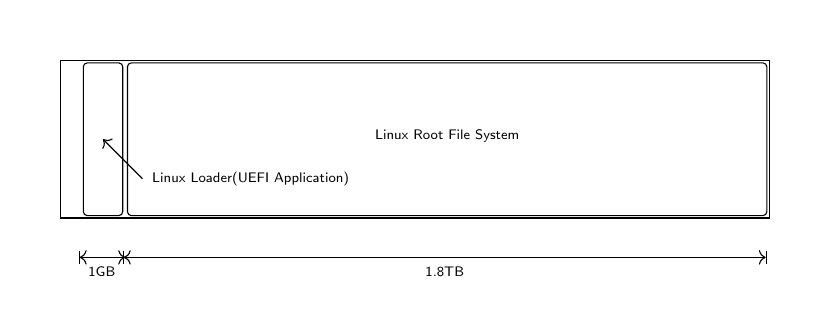
\begin{tikzpicture}[anchor=base,font=\tiny]
    {
      \pgfsetcornersarced{\pgfpoint{0.05cm}{0.05cm}}
      \uefipart
      \pgfusepath{stroke}
      % linux part
      \linuxpart
      \pgfusepath{stroke}
      \pgfsetcornersarced{\pgfpoint{0.0cm}{0.0cm}}
    }
    \begin{scope}
      \draw [|<->] (\uefiwixs, \partsizelocy)
        -- node[below] {1GB}
        (\uefiwixe, \partsizelocy);
      \draw [|<->|] (\linuxwixs, \partsizelocy)
        -- node[below] {1.8TB}
        (\linuxwixe, \partsizelocy);
    \end{scope}
    \begin{scope}
      \draw [<-] \uefind --
        ($(\uefixe, 0) 
          + 0.5*(0, \uefiys)
          + 0.5*(0, \uefiye)
          - 0.5*(0, \uefixe)
          + 0.5*(0, \uefixs)
          + (2.5mm, -2.5mm)$) 
          node[right]{Linux Loader(UEFI Application)};
      \node at \linuxnd {Linux Root File System};
    \end{scope}

    \begin{scope}[on background layer]
      % entire ssd
      \entirestr
      \pgfusepath{stroke}
      \outdentbounds
    \end{scope}
  \end{tikzpicture}
  \newpage
  % first partition
  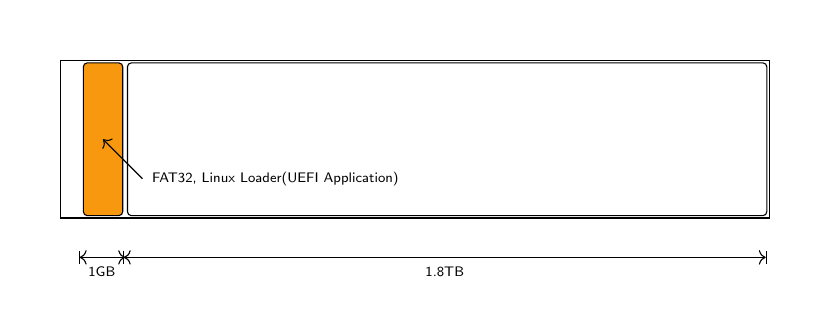
\begin{tikzpicture}[anchor=base,font=\tiny]
    {
      \pgfsetcornersarced{\pgfpoint{0.05cm}{0.05cm}}
      {
        \color{YellowOrange}
        \uefipart
        \pgfusepath{fill}
      }
      \uefipart
      \pgfusepath{stroke}
      % linux part
      \linuxpart
      \pgfusepath{stroke}
      \pgfsetcornersarced{\pgfpoint{0.0cm}{0.0cm}}
    }
    \begin{scope}
      \draw [|<->] (\uefiwixs, \partsizelocy)
        -- node[below] {1GB}
        (\uefiwixe, \partsizelocy);
      \draw [|<->|] (\linuxwixs, \partsizelocy)
        -- node[below] {1.8TB}
        (\linuxwixe, \partsizelocy);
    \end{scope}
    \begin{scope}
      \draw [color=CampbellBg,<-] \uefind --
        ($(\uefixe, 0) 
          + 0.5*(0, \uefiys)
          + 0.5*(0, \uefiye)
          - 0.5*(0, \uefixe)
          + 0.5*(0, \uefixs)$);
      \draw [] 
        ($(\uefixe, 0) 
          + 0.5*(0, \uefiys)
          + 0.5*(0, \uefiye)
          - 0.5*(0, \uefixe)
          + 0.5*(0, \uefixs)$) -- ++(2.5mm, -2.5mm);
      \node[right] 
        at ($(\uefixe, 0) 
          + 0.5*(0, \uefiys)
          + 0.5*(0, \uefiye)
          - 0.5*(0, \uefixe)
          + 0.5*(0, \uefixs)
          + (2.5mm, -2.5mm)$) 
        {FAT32, Linux Loader(UEFI Application)};
    \end{scope}
    \begin{scope}[on background layer]
      % entire ssd
      \entirestr
      \pgfusepath{stroke}
      \outdentbounds
    \end{scope}
  \end{tikzpicture}
  \newpage 
  % second partition
  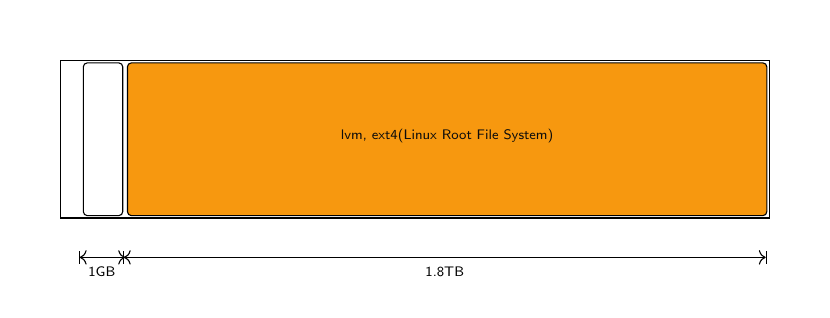
\begin{tikzpicture}[anchor=base,font=\tiny]
    {
      \pgfsetcornersarced{\pgfpoint{0.05cm}{0.05cm}}
      \uefipart
      \pgfusepath{stroke}
      % linux part
      {
        \color{YellowOrange}
        \linuxpart
        \pgfusepath{fill}
      }
      \linuxpart
      \pgfusepath{stroke}
      \pgfsetcornersarced{\pgfpoint{0.0cm}{0.0cm}}
    }
    \begin{scope}
      \draw [|<->] (\uefiwixs, \partsizelocy)
        -- node[below] {1GB}
        (\uefiwixe, \partsizelocy);
      \draw [|<->|] (\linuxwixs, \partsizelocy)
        -- node[below] {1.8TB}
        (\linuxwixe, \partsizelocy);
    \end{scope}
    \begin{scope}
      \node[color=CampbellBg] at \linuxnd {lvm, ext4(Linux Root File System)};
    \end{scope}

    \begin{scope}[on background layer]
      % entire ssd
      \entirestr
      \pgfusepath{stroke}
      \outdentbounds
    \end{scope}
  \end{tikzpicture}
  \newpage 
  % dark mbr
  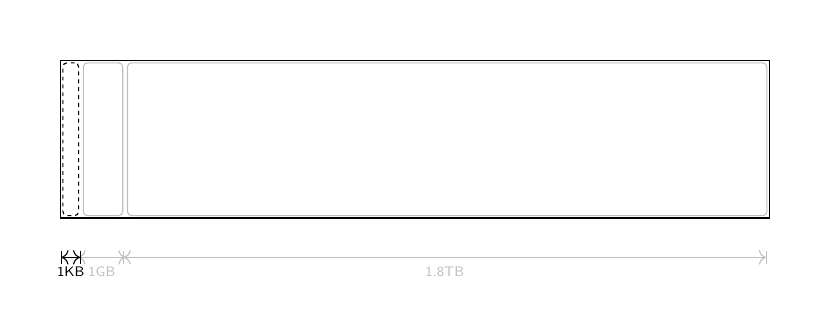
\begin{tikzpicture}[anchor=base,font=\tiny]
    \pgfsetcornersarced{\pgfpoint{0.05cm}{0.05cm}}
    % mbr part
    \pgfsetdash{{0.05cm}{0.05cm}}{0cm}
    \darkmbr
    \pgfusepath{stroke}
    \pgfsetcornersarced{\pgfpoint{0.0cm}{0.0cm}}
    \pgfsetdash{}{0cm}
    {
      \color{lightgray}
      \pgfsetcornersarced{\pgfpoint{0.05cm}{0.05cm}}
      % mbr part
      % uefi part
      \uefipart
      \pgfusepath{stroke}
      % linux part
      \linuxpart
      \pgfusepath{stroke}
      \pgfsetcornersarced{\pgfpoint{0.0cm}{0.0cm}}
    }
    \begin{scope}
      {
        \color{lightgray}
        \draw [<->] (\uefiwixs, \partsizelocy)
          -- node[below] {1GB}
          (\uefiwixe, \partsizelocy);
        \draw [|<->|] (\linuxwixs, \partsizelocy)
          -- node[below] {1.8TB}
          (\linuxwixe, \partsizelocy);
      }
      \draw [|<->|] (\mbrwixs, \partsizelocy)
        -- node[below] {1KB}
        (\mbrwixe, \partsizelocy);
    \end{scope}
    \begin{scope}[on background layer]
      % entire ssd
      \entirestr
      \pgfusepath{stroke}
      \outdentbounds
    \end{scope}
  \end{tikzpicture}
  \newpage
  % dark mbr
  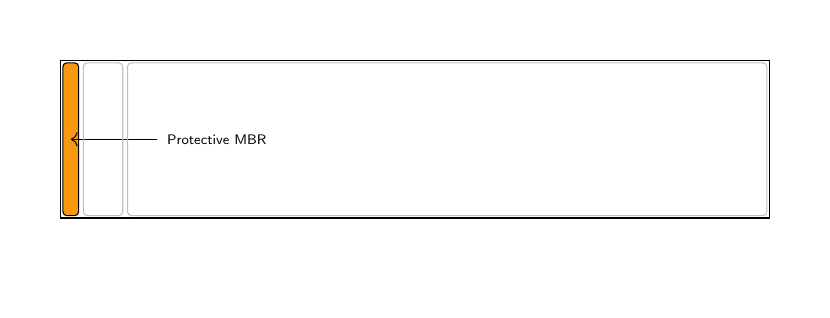
\begin{tikzpicture}[anchor=base,font=\tiny]
    \pgfsetcornersarced{\pgfpoint{0.05cm}{0.05cm}}
    % mbr part
    {
      \color{YellowOrange}
      \darkmbr
      \pgfusepath{fill}
    }
    \darkmbr
    \pgfusepath{stroke}

    \draw[<-,color=CampbellBg]
      ($0.5*(\mbrxs, \mbrys) + 0.5*(\mbrxe, \mbrye)$)
      -- ($0.5*(\mbrxs, \mbrys)
        + 0.5*(\mbrxe, \mbrye)
        + 0.5*(\mbrxe, 0)
        - 0.5*(\mbrxs, 0)$);

    \draw[]
      ($0.5*(\mbrxs, \mbrys)
        + 0.5*(\mbrxe, \mbrye)
        + 0.5*(\mbrxe, 0)
        - 0.5*(\mbrxs, 0)$)
      -- ++(1cm, 0) node[right] {Protective MBR};

    \pgfsetcornersarced{\pgfpoint{0.0cm}{0.0cm}}
    {
      \color{lightgray}
      \pgfsetcornersarced{\pgfpoint{0.05cm}{0.05cm}}
      % mbr part
      % uefi part
      \uefipart
      \pgfusepath{stroke}
      % linux part
      \linuxpart
      \pgfusepath{stroke}
      \pgfsetcornersarced{\pgfpoint{0.0cm}{0.0cm}}
    }
    \begin{scope}[on background layer]
      % entire ssd
      \entirestr
      \pgfusepath{stroke}
      \outdentbounds
    \end{scope}
  \end{tikzpicture}
\end{document} 
% vi: se ts=2 sw=2 et:
